\documentclass{beamer}
\usetheme{Madrid}
\usecolortheme{default}
\usepackage{tikz}
\usepackage{amsmath}
\usetikzlibrary{arrows.meta, positioning, shapes.geometric, calc, decorations.pathreplacing, fit, backgrounds}

\title{Optimizing Attention Mechanisms}
\subtitle{Flash Attention and Paged Attention}
\author{CS677: Parallel Programming}
\date{\today}

\begin{document}

\frame{\titlepage}

% ===== SLIDE 1: Problem Statement =====
\begin{frame}{Suitability for GPU Acceleration}
    \begin{itemize}
        \item Attention is the core of Transformer models: $O = \text{softmax}\!\left(\frac{QK^T}{\sqrt{d}}\right)V$.
        \item Dominated by large matrix multiplications ($QK^T$, $PV$) --- highly parallel and well-suited to GPU SIMT execution.
        \item However, it is \textbf{memory bandwidth-bound}, not compute-bound: the arithmetic intensity is low relative to the data movement required.
        \item The attention matrix $S = QK^T$ has size $O(N^2)$, where $N$ is the sequence length.
        \item Moving $O(N^2)$ intermediate data to/from \textbf{Global Memory (HBM)} causes a severe bottleneck: HBM bandwidth (${\sim}2$\,TB/s) is orders of magnitude slower than on-chip SRAM, making na\"ive implementations spend most time waiting on memory rather than computing.
        \item As $N$ grows (e.g.\ 2K $\to$ 128K context), the $O(N^2)$ traffic dominates wall-clock time and can exceed available GPU memory entirely.
    \end{itemize}
\end{frame}

% ===== SLIDE 2: Naive Attention with clear 3-kernel pipeline =====
\begin{frame}{Naive Attention: The Three-Kernel Pipeline}
    \begin{center}
    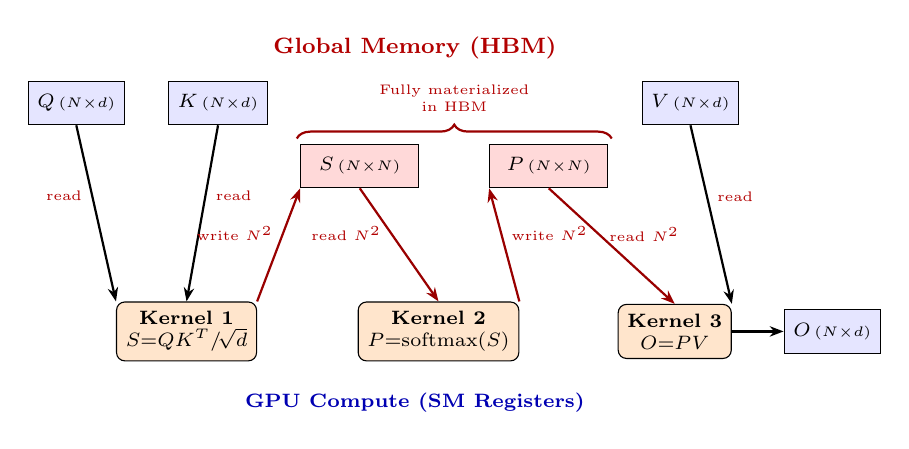
\begin{tikzpicture}[
        tensor/.style={draw, rectangle, fill=blue!10, minimum width=1.2cm, minimum height=0.55cm, align=center, font=\scriptsize},
        big/.style={draw, rectangle, fill=red!15, minimum width=1.5cm, minimum height=0.55cm, align=center, font=\scriptsize},
        op/.style={draw, rounded corners=3pt, fill=orange!20, minimum width=1.4cm, minimum height=0.55cm, align=center, font=\scriptsize},
        hbmbox/.style={draw, dashed, rounded corners, fill=red!3, inner sep=6pt},
        arrow/.style={-{Stealth[length=5pt]}, thick},
        iolabel/.style={font=\tiny, color=red!70!black}
    ]
        % --- HBM region label ---
        \node[font=\footnotesize\bfseries, color=red!70!black] at (0.5, 3.3) {Global Memory (HBM)};

        % --- Row 1: Inputs in HBM ---
        \node[tensor] (Q) at (-3.8, 2.6) {$Q$\,\tiny$(N{\times}d)$};
        \node[tensor] (K) at (-2.0, 2.6) {$K$\,\tiny$(N{\times}d)$};
        \node[tensor] (V) at (4.0, 2.6) {$V$\,\tiny$(N{\times}d)$};

        % --- Intermediate materialized matrices ---
        \node[big] (S) at (-0.2, 1.8) {$S$\,\tiny$(N{\times}N)$};
        \node[big] (P) at (2.2, 1.8) {$P$\,\tiny$(N{\times}N)$};

        % --- Output ---
        \node[tensor] (O) at (5.8, -0.3) {$O$\,\tiny$(N{\times}d)$};

        % --- Three separate GPU kernels ---
        \node[op] (k1) at (-2.4, -0.3) {\textbf{Kernel 1}\\$S{=}QK^T/\!\sqrt{d}$};
        \node[op] (k2) at (0.8, -0.3) {\textbf{Kernel 2}\\$P{=}\text{softmax}(S)$};
        \node[op] (k3) at (3.8, -0.3) {\textbf{Kernel 3}\\$O{=}PV$};

        \node[font=\scriptsize\bfseries, color=blue!70!black] at (0.5, -1.2) {GPU Compute (SM Registers)};

        % --- Data flow arrows ---
        % Kernel 1: read Q,K from HBM, write S to HBM
        \draw[arrow] (Q.south) -- (k1.north west) node[pos=0.4, left, iolabel] {read};
        \draw[arrow] (K.south) -- (k1.north) node[pos=0.4, right, iolabel] {read};
        \draw[arrow, color=red!60!black] (k1.north east) -- (S.south west) node[pos=0.6, left, iolabel] {write $N^2$};

        % Kernel 2: read S from HBM, write P to HBM
        \draw[arrow, color=red!60!black] (S.south) -- (k2.north) node[pos=0.4, left, iolabel] {read $N^2$};
        \draw[arrow, color=red!60!black] (k2.north east) -- (P.south west) node[pos=0.6, right, iolabel] {write $N^2$};

        % Kernel 3: read P,V from HBM, write O to HBM
        \draw[arrow, color=red!60!black] (P.south) -- (k3.north) node[pos=0.4, right, iolabel] {read $N^2$};
        \draw[arrow] (V.south) -- (k3.north east) node[pos=0.4, right, iolabel] {read};
        \draw[arrow] (k3.east) -- (O.west);

        % --- Brace showing total HBM traffic ---
        \draw[decorate, decoration={brace, amplitude=5pt}, thick, red!60!black]
            (-1.0, 2.15) -- (3.0, 2.15) node[midway, above=6pt, font=\tiny, color=red!70!black, align=center] {Fully materialized\\in HBM};

    \end{tikzpicture}
    \end{center}

    \vspace{0.1cm}
    \small
    \textbf{Bottleneck:} Three separate kernel launches. $S$ and $P$ (each $N{\times}N$) are fully written to and read from slow HBM between every step, totaling $\mathbf{4N^2}$ HBM transfers.
\end{frame}

% ===== SLIDE 3: Flash Attention -- Tiling Overview =====
\begin{frame}{Flash Attention: Tiling Strategy}
    \begin{center}
    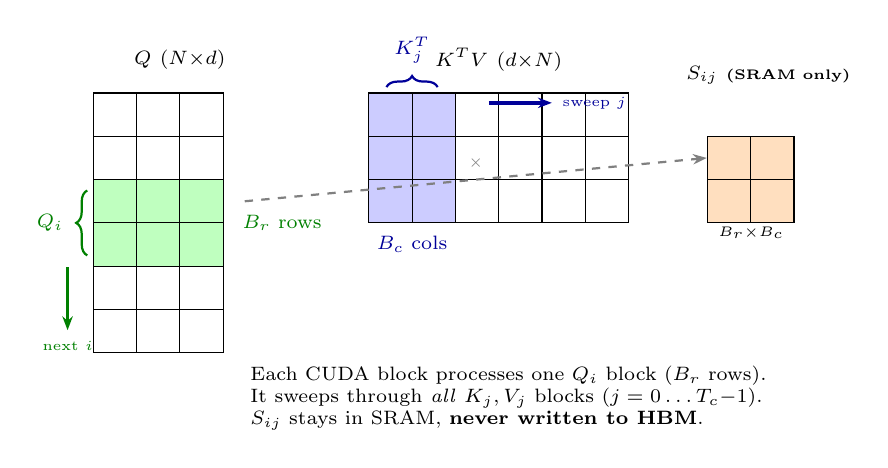
\begin{tikzpicture}[
        cell/.style={draw, minimum width=0.55cm, minimum height=0.55cm, font=\tiny},
        highlight/.style={fill=green!25},
        khighlight/.style={fill=blue!20},
        arrow/.style={-{Stealth[length=5pt]}, thick}
    ]
        % --- Q matrix ---
        % Label centered above the matrix
        \node[font=\scriptsize\bfseries] at (-3.675, 2.7) {$Q$ $(N{\times}d)$};
        \foreach \r in {0,...,5} {
            \foreach \c in {0,...,2} {
                \node[cell] at (-4.5+\c*0.55, 2-\r*0.55) {};
            }
        }
        % Highlight Q_i block (rows 2-3)
        \foreach \c in {0,...,2} {
            \node[cell, highlight] at (-4.5+\c*0.55, 2-2*0.55) {};
            \node[cell, highlight] at (-4.5+\c*0.55, 2-3*0.55) {};
        }
        % Brace on left side pointing inward (mirror = opens right toward matrix)
        \draw[decorate, decoration={brace, amplitude=4pt, mirror}, thick, green!50!black]
            (-4.85, 2-1.75*0.55) -- (-4.85, 2-3.25*0.55) node[midway, left=5pt, font=\scriptsize\bfseries, color=green!50!black] {$Q_i$};
        \node[font=\scriptsize, color=green!50!black, anchor=west] at (-3, 2-2.5*0.55) {$B_r$ rows};

        % --- K^T matrix ---
        % Label centered above the matrix
        \node[font=\scriptsize\bfseries] at (0.375, 2.7) {$K^TV$ $(d{\times}N)$};
        \foreach \r in {0,...,2} {
            \foreach \c in {0,...,5} {
                \node[cell] at (-1+\c*0.55, 2-\r*0.55) {};
            }
        }
        % Highlight K_j block (cols 0-1)
        \foreach \r in {0,...,2} {
            \node[cell, khighlight] at (-1+0*0.55, 2-\r*0.55) {};
            \node[cell, khighlight] at (-1+1*0.55, 2-\r*0.55) {};
        }
        % Brace on top pointing inward (no mirror = opens downward toward matrix)
        \draw[decorate, decoration={brace, amplitude=4pt}, thick, blue!60!black]
            (-1-0.05, 2+0.35) -- (-1+1*0.55+0.05, 2+0.35) node[midway, above=5pt, font=\scriptsize\bfseries, color=blue!60!black] {$K_j^T$};
        \node[font=\scriptsize, color=blue!60!black] at (-0.725, 0.35) {$B_c$ cols};

        % --- Result S_ij (small block, never in HBM) ---
        \node[font=\scriptsize\bfseries] at (3.8, 2.5) {$S_{ij}$ \tiny(SRAM only)};
        \node[cell, fill=orange!25] (s00) at (3.3, 1.45) {};
        \node[cell, fill=orange!25] (s01) at (3.85, 1.45) {};
        \node[cell, fill=orange!25] (s10) at (3.3, 0.9) {};
        \node[cell, fill=orange!25] (s11) at (3.85, 0.9) {};
        \node[font=\tiny] at (3.58, 0.5) {$B_r{\times}B_c$};

        % Arrow from Q_i x K_j -> S_ij
        \draw[arrow, dashed, gray] (-2.85, 0.9) -- (s00.west) node[midway, above, font=\tiny] {$\times$};

        % --- Iteration arrows ---
        \draw[arrow, blue!60!black, very thick] (-1+2*0.55+0.15, 2.15) -- (-1+3*0.55+0.4, 2.15) node[right, font=\tiny, color=blue!60!black] {sweep $j$};
        \draw[arrow, green!50!black, very thick] (-5.1, 2-3.25*0.55-0.15) -- (-5.1, 2-4.25*0.55-0.4) node[below, font=\tiny, color=green!50!black] {next $i$};

        % --- Legend ---
        \node[font=\scriptsize, align=left] at (0.5, -1.6) {
            Each CUDA block processes one $Q_i$ block ($B_r$ rows).\\
            It sweeps through \emph{all} $K_j, V_j$ blocks ($j = 0 \ldots T_c{-}1$).\\
            $S_{ij}$ stays in SRAM, \textbf{never written to HBM}.
        };

    \end{tikzpicture}
    \end{center}
\end{frame}

% ===== SLIDE 4: Flash Attention -- Online Softmax =====
\begin{frame}{Flash Attention: Online Softmax Trick}
    \small
    \textbf{Problem:} Softmax needs the global max over all $N$ keys, but we only see $B_c$ at a time.

    \vspace{0.1cm}
    \begin{center}
    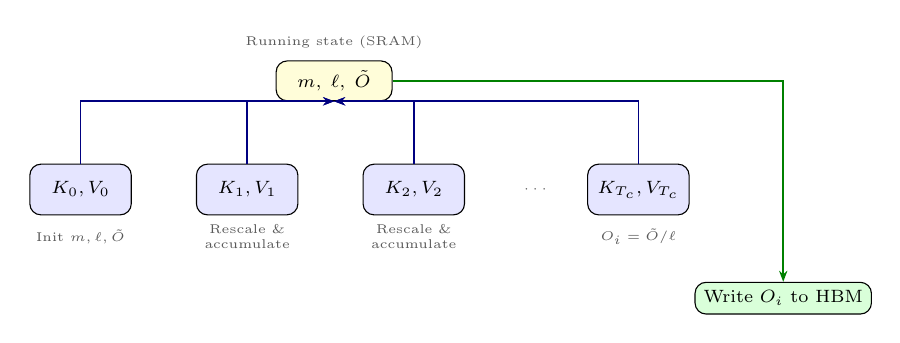
\begin{tikzpicture}[scale=0.92, every node/.style={transform shape},
        kblock/.style={draw, rounded corners, fill=blue!10, minimum width=1.4cm, minimum height=0.7cm, align=center, font=\scriptsize},
        state/.style={draw, rounded corners, fill=yellow!15, minimum width=1.6cm, minimum height=0.55cm, align=center, font=\scriptsize},
        arrow/.style={-{Stealth[length=4pt]}, semithick},
        note/.style={font=\tiny, color=gray!70!black, align=center}
    ]
        % Running state register (top)
        \node[state] (s0) at (0, 1.5) {$m,\;\ell,\;\tilde{O}$};
        \node[note, above=1pt] at (s0.north) {Running state (SRAM)};

        % K/V blocks (bottom row)
        \node[kblock] (k0) at (-3.5, 0) {$K_0, V_0$};
        \node[kblock] (k1) at (-1.2, 0) {$K_1, V_1$};
        \node[kblock] (k2) at (1.1, 0) {$K_2, V_2$};
        \node[note]        at (2.8, 0) {$\cdots$};
        \node[kblock] (kT) at (4.2, 0) {$K_{T_c}, V_{T_c}$};

        % Arrows from each block up to the state
        \foreach \kb in {k0, k1, k2, kT} {
            \draw[arrow, blue!50!black] (\kb.north) -- (s0.south -| \kb.north) -- (s0.south);
        }

        % Update steps as annotations below blocks
        \node[note] at (-3.5, -0.65) {Init $m, \ell, \tilde{O}$};
        \node[note] at (-1.2, -0.65) {Rescale \&\\accumulate};
        \node[note] at (1.1, -0.65) {Rescale \&\\accumulate};
        \node[note] at (4.2, -0.65) {$O_i = \tilde{O}/\ell$};

        % Output
        \node[draw, fill=green!15, rounded corners, font=\scriptsize] (out) at (6.2, -1.5) {Write $O_i$ to HBM};
        \draw[arrow, green!50!black] (s0.east) -| (out.north);

    \end{tikzpicture}
    \end{center}

    \vspace{-0.05cm}
    \footnotesize
    Three values maintained per row in SRAM: \;$m$ (running max), \;$\ell$ (softmax denominator), \;$\tilde{O}$ (output accumulator).

    \vspace{0.1cm}
    On each new block: if a larger score appears, rescale prior work by $e^{m_{\text{old}} - m_{\text{new}}}$, then accumulate. Final: $O_i = \tilde{O} / \ell$.
\end{frame}

% ===== SLIDE 5: Flash Attention -- Full Data Flow =====
\begin{frame}{Flash Attention: Fused Single-Kernel Data Flow}
    \begin{center}
    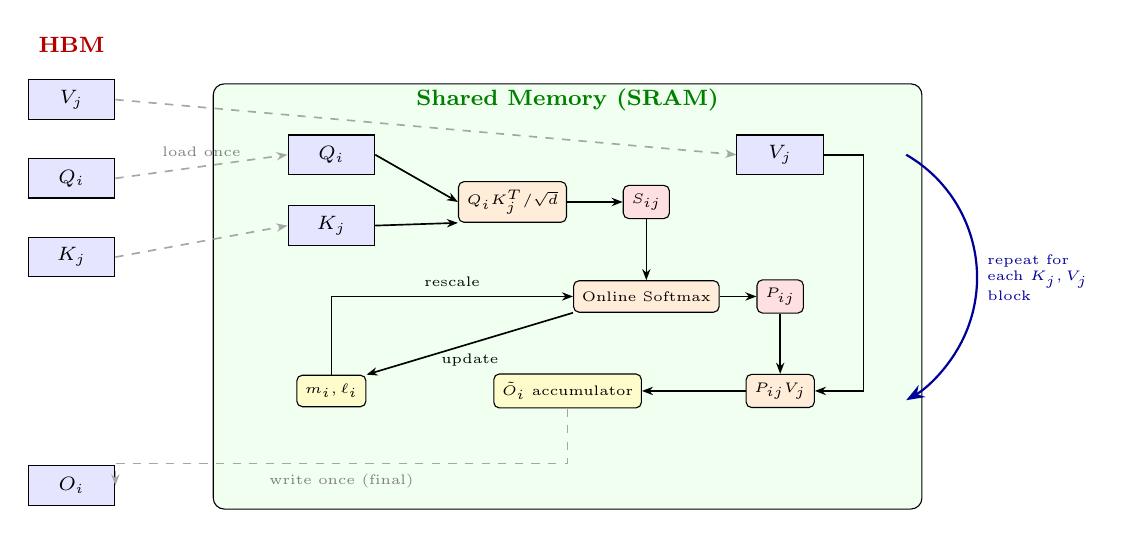
\begin{tikzpicture}[
        tensor/.style={draw, rectangle, fill=blue!10, minimum width=1.1cm, minimum height=0.5cm, font=\scriptsize},
        op/.style={draw, rounded corners=2pt, fill=orange!15, minimum height=0.4cm, align=center, font=\tiny, inner sep=3pt},
        acc/.style={draw, rounded corners=2pt, fill=yellow!20, minimum height=0.4cm, align=center, font=\tiny, inner sep=3pt},
        arrow/.style={-{Stealth[length=4pt]}, semithick},
        dasharrow/.style={-{Stealth[length=4pt]}, semithick, dashed, color=gray!70}
    ]
        % --- HBM region (left column) ---
        \node[font=\footnotesize\bfseries, color=red!70!black] at (-3.8, 3.4) {HBM};
        \node[tensor] (Vj_hbm) at (-3.8, 2.7) {$V_j$};
        \node[tensor] (Qi_hbm) at (-3.8, 1.7) {$Q_i$};
        \node[tensor] (Kj_hbm) at (-3.8, 0.7) {$K_j$};
        \node[tensor] (Oi_hbm) at (-3.8, -2.2) {$O_i$};

        % --- SRAM box ---
        \node[draw, rounded corners, fill=green!6, minimum width=9.0cm, minimum height=5.4cm] (sram) at (2.5, 0.2) {};
        \node[font=\footnotesize\bfseries, color=green!50!black] at (2.5, 2.7) {Shared Memory (SRAM)};

        % --- SRAM contents: inputs (V_j on top, then Q_i, K_j) ---
        \node[tensor] (Vj_s) at (5.2, 2.0) {$V_j$};
        \node[tensor] (Qi_s) at (-0.5, 2.0) {$Q_i$};
        \node[tensor] (Kj_s) at (-0.5, 1.1) {$K_j$};

        % --- Compute pipeline ---
        \node[op] (matmul) at (1.8, 1.4) {$Q_i K_j^T / \sqrt{d}$};
        \node[op, fill=red!12] (sij) at (3.5, 1.4) {$S_{ij}$};
        \node[op] (osm) at (3.5, 0.2) {Online Softmax};
        \node[op, fill=red!12] (pij) at (5.2, 0.2) {$P_{ij}$};
        \node[op] (mm2) at (5.2, -1.0) {$P_{ij} V_j$};

        % --- Accumulators ---
        \node[acc] (acc) at (2.5, -1.0) {$\tilde{O}_i$ accumulator};
        \node[acc] (stats) at (-0.5, -1.0) {$m_i, \ell_i$};

        % --- HBM -> SRAM load arrows ---
        \draw[dasharrow] (Qi_hbm.east) -- (Qi_s.west) node[midway, above, font=\tiny, color=gray] {load once};
        \draw[dasharrow] (Kj_hbm.east) -- (Kj_s.west);
        \draw[dasharrow] (Vj_hbm.east) -- (Vj_s.west);

        % --- Internal compute arrows ---
        \draw[arrow] (Qi_s.east) -- (matmul.west);
        \draw[arrow] (Kj_s.east) -- (matmul.south west);
        \draw[arrow] (matmul.east) -- (sij.west);
        \draw[arrow] (sij.south) -- (osm.north);
        \draw[arrow] (osm.east) -- (pij.west);
        \draw[arrow] (pij.south) -- (mm2.north);
        \draw[arrow] (Vj_s.east) -- ++(0.5, 0) |- (mm2.east);
        \draw[arrow] (mm2.west) -- (acc.east);

        % --- Online softmax state loop ---
        \draw[arrow] (osm.south west) -- (stats.north east) node[midway, below, font=\tiny] {update};
        \draw[arrow] (stats.north) |- (osm.west) node[pos=0.75, above, font=\tiny] {rescale};

        % --- Write back to HBM ---
        \draw[dasharrow] (acc.south) -- ++(0, -0.7) -| (Oi_hbm.east) node[pos=0.25, below, font=\tiny, color=gray] {write once (final)};

        % --- Loop annotation ---
        \draw[thick, blue!60!black, -{Stealth}] (6.8, 2.0) arc[start angle=60, end angle=-60, radius=1.8cm]
            node[midway, right, font=\tiny, color=blue!60!black, align=left] {repeat for\\each $K_j, V_j$\\block};

    \end{tikzpicture}
    \end{center}

    \vspace{-0.1cm}
    \footnotesize
    \textbf{Single kernel.} $Q_i$ loaded once; $K_j, V_j$ stream through SRAM. The $N{\times}N$ matrix is \textbf{never materialized} in HBM. HBM traffic: $O(N)$ per query block.
\end{frame}

% ===== SLIDE 6: Flash Attention Results =====
\begin{frame}{Flash Attention: Results}
    \begin{table}[]
    \centering
    \resizebox{\columnwidth}{!}{%
    \begin{tabular}{|l|c|c|c|}
    \hline
    \textbf{Config ($N$)} & \textbf{Optimized PyTorch} & \textbf{Flash (Ours)} & \textbf{Na\"ive Benchmark} \\ \hline
    B=1 H=1 N=64         & 98.3 $\mu$s                & 66.7 $\mu$s           & 79.2 $\mu$s               \\
    B=1 H=4 N=256        & 93.9 $\mu$s                & 418.4 $\mu$s          & 591.7 $\mu$s              \\
    B=4 H=8 N=1024       & 1.52 ms                    & 17.34 ms              & 42.18 ms                  \\
    B=4 H=8 N=2048       & 6.21 ms                    & 91.47 ms              & 387.6 ms                  \\ \hline
    \end{tabular}%
    }
    \caption{Latency comparison: optimized PyTorch vs our Flash kernel vs na\"ive attention}
    \end{table}
    \begin{itemize}
        \item \textbf{Vanilla} is the highly optimized PyTorch/cuBLAS fused implementation---our pedagogical kernel is not expected to match it.
        \item \textbf{Na\"ive benchmark:} Un-fused three-kernel attention (no tiling). Our Flash kernel is ${\sim}1.2$--$4.2{\times}$ faster, with the gap widening at larger $N$ as the $O(N^2)$ HBM traffic dominates.
        \item At $N{=}2048$ the na\"ive path is $\mathbf{4.2{\times}}$ slower than our kernel, consistent with published Flash Attention speedups at longer sequences.
    \end{itemize}
\end{frame}

% ===== SLIDE 7: Paged Attention -- Motivation =====
\begin{frame}{Paged Attention: Tackling KV Cache Fragmentation}
    \begin{center}
    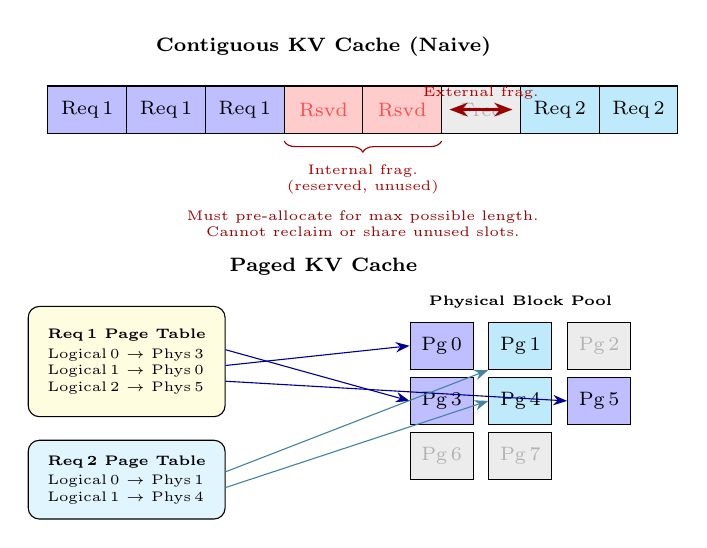
\begin{tikzpicture}[
        cell/.style={draw, rectangle, minimum width=1.0cm, minimum height=0.6cm, font=\scriptsize},
        used/.style={fill=blue!25},
        unused/.style={fill=gray!15, text=gray!60},
        reserved/.style={fill=red!20},
        arrow/.style={-{Stealth[length=5pt]}, thick}
    ]
        % === Naive contiguous layout ===
        \node[font=\scriptsize\bfseries] at (0, 3.2) {Contiguous KV Cache (Naive)};

        \node[cell, used]     at (-3.0, 2.4) {Req\,1};
        \node[cell, used]     at (-2.0, 2.4) {Req\,1};
        \node[cell, used]     at (-1.0, 2.4) {Req\,1};
        \node[cell, reserved] at ( 0.0, 2.4) {\color{red!70}Rsvd};
        \node[cell, reserved] at ( 1.0, 2.4) {\color{red!70}Rsvd};
        \node[cell, unused]   at ( 2.0, 2.4) {Free};
        \node[cell, used, fill=cyan!25] at ( 3.0, 2.4) {Req\,2};
        \node[cell, used, fill=cyan!25] at ( 4.0, 2.4) {Req\,2};

        % Annotations
        \draw[decorate, decoration={brace, amplitude=4pt, mirror}, red!60!black]
            (-0.5, 2.0) -- (1.5, 2.0) node[midway, below=5pt, font=\tiny, color=red!70!black, align=center] {Internal frag.\\(reserved, unused)};
        \draw[{Stealth}-{Stealth}, red!60!black, thick] (1.6, 2.4) -- (2.4, 2.4)
            node[midway, above, font=\tiny, color=red!70!black] {External frag.};

        \node[font=\tiny, color=red!60!black, align=center] at (0.5, 0.95) {Must pre-allocate for max possible length.\\Cannot reclaim or share unused slots.};

        % === Paged layout ===
        \node[font=\scriptsize\bfseries] at (0, 0.4) {Paged KV Cache};

        % Page Table for Req 1
        \node[draw, fill=yellow!12, rounded corners, minimum width=2.5cm, minimum height=1.4cm, align=left, font=\tiny, inner sep=4pt] (pt1) at (-2.5, -0.8)
            {\textbf{Req\,1 Page Table}\\[1pt]
             Logical\,0 $\to$ Phys\,3\\
             Logical\,1 $\to$ Phys\,0\\
             Logical\,2 $\to$ Phys\,5};

        % Page Table for Req 2
        \node[draw, fill=cyan!12, rounded corners, minimum width=2.5cm, minimum height=1.0cm, align=left, font=\tiny, inner sep=4pt] (pt2) at (-2.5, -2.3)
            {\textbf{Req\,2 Page Table}\\[1pt]
             Logical\,0 $\to$ Phys\,1\\
             Logical\,1 $\to$ Phys\,4};

        % Physical block pool
        \node[font=\tiny\bfseries] at (2.5, -0.05) {Physical Block Pool};
        \node[cell, used, minimum width=0.8cm] (p0) at (1.5, -0.6) {Pg\,0};
        \node[cell, used, fill=cyan!25, minimum width=0.8cm] (p1) at (2.5, -0.6) {Pg\,1};
        \node[cell, unused, minimum width=0.8cm] (p2) at (3.5, -0.6) {Pg\,2};
        \node[cell, used, minimum width=0.8cm] (p3) at (1.5, -1.3) {Pg\,3};
        \node[cell, used, fill=cyan!25, minimum width=0.8cm] (p4) at (2.5, -1.3) {Pg\,4};
        \node[cell, used, minimum width=0.8cm] (p5) at (3.5, -1.3) {Pg\,5};
        \node[cell, unused, minimum width=0.8cm] (p6) at (1.5, -2.0) {Pg\,6};
        \node[cell, unused, minimum width=0.8cm] (p7) at (2.5, -2.0) {Pg\,7};

        % Arrows from page tables to physical blocks
        \draw[arrow, blue!60!black, thin] ([yshift=0.15cm]pt1.east) -- (p3.west);
        \draw[arrow, blue!60!black, thin] ([yshift=-0.05cm]pt1.east) -- (p0.west);
        \draw[arrow, blue!60!black, thin] ([yshift=-0.25cm]pt1.east) -- (p5.west);
        \draw[arrow, cyan!60!black, thin] ([yshift=0.1cm]pt2.east) -- (p1.south west);
        \draw[arrow, cyan!60!black, thin] ([yshift=-0.1cm]pt2.east) -- (p4.west);

    \end{tikzpicture}
    \end{center}

    \vspace{-0.1cm}
    \footnotesize
    \textbf{Key idea:} Borrow OS virtual memory paging. Each request's KV cache maps through a per-request \textbf{page table} to \emph{non-contiguous} physical blocks. Blocks are allocated on-demand and freed immediately, eliminating fragmentation.
\end{frame}

% ===== SLIDE 8: Paged Attention -- Kernel Design =====
\begin{frame}{Paged Attention: Kernel Design (V1 vs V2)}
    \begin{center}
    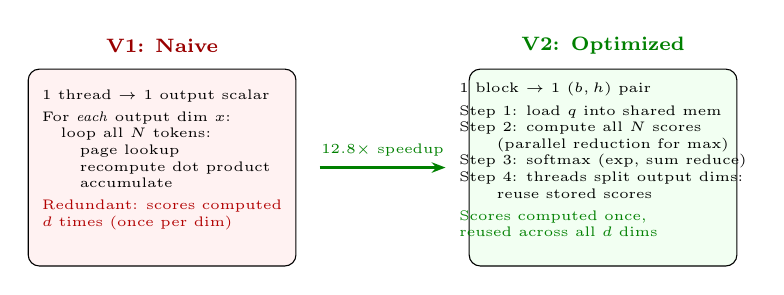
\begin{tikzpicture}[
        box/.style={draw, rounded corners, minimum width=3.4cm, minimum height=2.5cm, align=center, font=\scriptsize},
        stepbox/.style={font=\tiny, align=left},
        arrow/.style={-{Stealth[length=5pt]}, thick}
    ]
        % V1
        \node[box, fill=red!5] (v1) at (-2.8, 0) {};
        \node[font=\scriptsize\bfseries, color=red!60!black] at (-2.8, 1.55) {V1: Naive};
        \node[stepbox] at (-2.8, 0.1) {
            1 thread $\to$ 1 output scalar\\[2pt]
            For \emph{each} output dim $x$:\\
            \quad loop all $N$ tokens:\\
            \quad\quad page lookup\\
            \quad\quad recompute dot product\\
            \quad\quad accumulate\\[2pt]
            \textcolor{red!70!black}{Redundant: scores computed}\\
            \textcolor{red!70!black}{$d$ times (once per dim)}
        };

        % Arrow
        \draw[arrow, very thick, green!50!black] (-0.8, 0) -- (0.8, 0)
            node[midway, above, font=\tiny, color=green!50!black] {$12.8\times$ speedup};

        % V2
        \node[box, fill=green!5] (v2) at (2.8, 0) {};
        \node[font=\scriptsize\bfseries, color=green!50!black] at (2.8, 1.55) {V2: Optimized};
        \node[stepbox] at (2.8, 0.1) {
            1 block $\to$ 1 $(b, h)$ pair\\[2pt]
            Step 1: load $q$ into shared mem\\
            Step 2: compute all $N$ scores\\
            \quad\quad (parallel reduction for max)\\
            Step 3: softmax (exp, sum reduce)\\
            Step 4: threads split output dims:\\
            \quad\quad reuse stored scores\\[2pt]
            \textcolor{green!50!black}{Scores computed once,}\\
            \textcolor{green!50!black}{reused across all $d$ dims}
        };

    \end{tikzpicture}
    \end{center}

    \vspace{0.1cm}
    \footnotesize
    \textbf{V2 wins by:} (1) computing attention scores \emph{once} and reusing them, (2) cooperative thread-block reductions for max/sum, and (3) coalesced global memory reads via block-level parallelism.
\end{frame}

% ===== SLIDE 9: Paged Attention Results =====
\begin{frame}{Paged Attention: Results}
    \begin{table}[]
    \centering
    \resizebox{\columnwidth}{!}{%
    \begin{tabular}{|l|c|c|c|}
    \hline
    \textbf{Implementation} & \textbf{Latency/fwd} & \textbf{Fwd/s} & \textbf{Rows/s} \\ \hline
    Paged v1               & 2.58 ms             & 388.0          & 1,552.2       \\
    Paged v2               & 200.1 $\mu$s        & 4,996.4        & 19,985.7      \\ \hline
    \end{tabular}%
    }
    \caption{Paged Attention Throughput (Config: B=4, H=8, d=64, N=512)}
    \end{table}
    \textbf{V2 achieves a $\mathbf{12.8\times}$ speedup} by eliminating redundant score computation and leveraging cooperative thread-block reductions with coalesced memory access.
\end{frame}

% ===== SLIDE 10: GPT-2 End-to-End Integration =====
\begin{frame}{End-to-End Integration: GPT-2}
    \begin{center}
    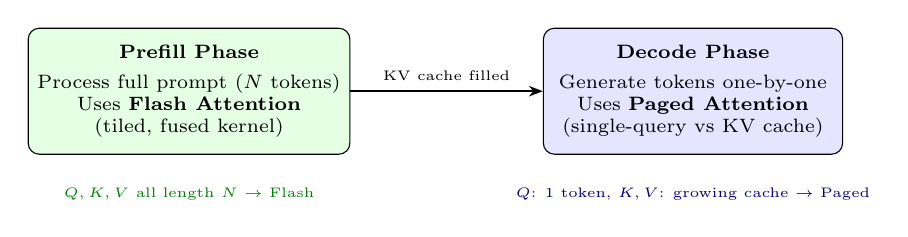
\begin{tikzpicture}[
        phase/.style={draw, rounded corners, minimum width=3.8cm, minimum height=1.6cm, align=center, font=\scriptsize},
        arrow/.style={-{Stealth[length=5pt]}, thick}
    ]
        % Prefill
        \node[phase, fill=green!10] (prefill) at (-3.2, 0) {
            \textbf{Prefill Phase}\\[3pt]
            Process full prompt ($N$ tokens)\\
            Uses \textbf{Flash Attention}\\
            (tiled, fused kernel)
        };

        % Decode
        \node[phase, fill=blue!10] (decode) at (3.2, 0) {
            \textbf{Decode Phase}\\[3pt]
            Generate tokens one-by-one\\
            Uses \textbf{Paged Attention}\\
            (single-query vs KV cache)
        };

        \draw[arrow] (prefill) -- (decode) node[midway, above, font=\tiny] {KV cache filled};

        % Labels
        \node[font=\tiny, color=green!50!black] at (-3.2, -1.3) {$Q,K,V$ all length $N$ $\to$ Flash};
        \node[font=\tiny, color=blue!50!black] at (3.2, -1.3) {$Q$: 1 token, $K,V$: growing cache $\to$ Paged};

    \end{tikzpicture}
    \end{center}

    \vspace{0.3cm}
    \begin{table}[]
    \centering
    \resizebox{\columnwidth}{!}{%
    \begin{tabular}{|l|c|c|}
    \hline
    \textbf{Variant} & \textbf{Prefill (N=512) Latency} & \textbf{End-to-End TPS} \\ \hline
    Standard HuggingFace  & 10.99 ms                        & 114.20 tokens/sec       \\
    Custom CUDA Kernels   & 11.04 ms                        & 112.29 tokens/sec       \\ \hline
    \end{tabular}%
    }
    \end{table}
    \footnotesize
    \textbf{Performance parity} with PyTorch/HuggingFace confirms correctness of both custom kernels when integrated into a real model's inference pipeline.
\end{frame}

\end{document}
